% Flow diagram for ISP process - TikZ
% Compile with: pdflatex diagrama_flujo.tex
\documentclass[tikz,border=3pt]{standalone}
\usepackage[utf8]{inputenc}
\usepackage[T1]{fontenc}
\usepackage{amsmath}
\usepackage{mathptmx}
\usetikzlibrary{shapes,arrows,positioning}

\begin{document}
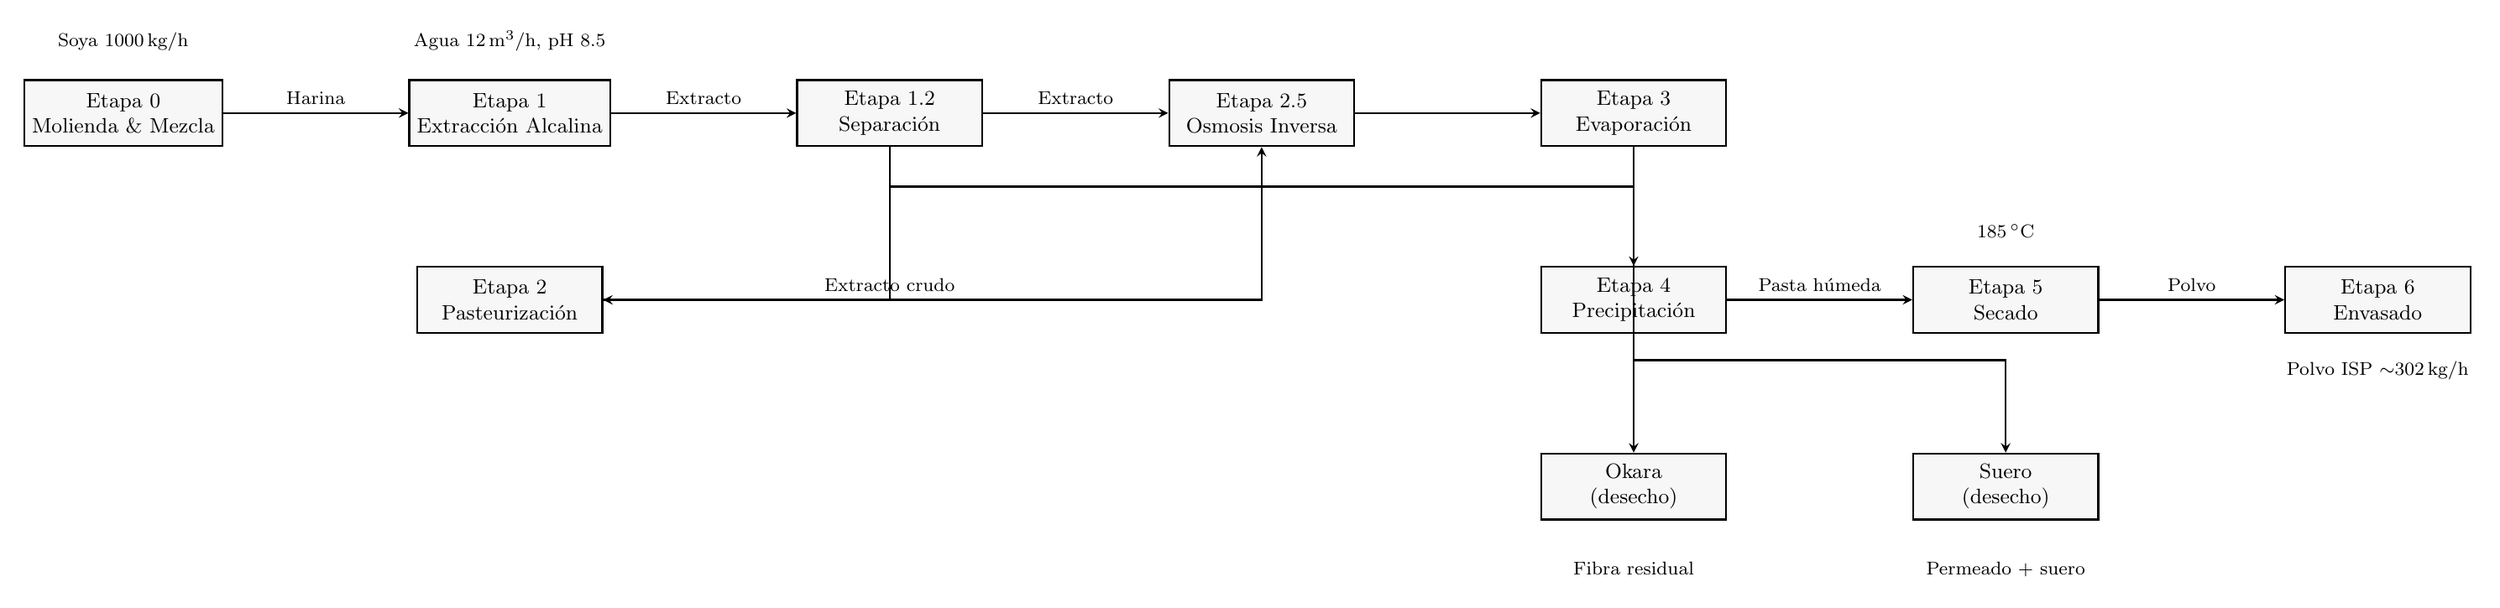
\begin{tikzpicture}[
    node distance=1.8cm and 2.8cm,
    box/.style={
        rectangle, draw, minimum width=2.8cm, minimum height=1.0cm,
        align=center, font=\small, fill=black!3, thick
    },
    arrow/.style={->, thick, >=stealth},
    label/.style={font=\footnotesize, above}
]

% Nodes
\node[box] (E0)  {Etapa 0\\Molienda \& Mezcla};
\node[box, right=of E0] (E1) {Etapa 1\\Extracci\'on Alcalina};
\node[box, right=of E1] (E1b) {Etapa 1.2\\Separaci\'on};
\node[box, below=of E1] (E2) {Etapa 2\\Pasteurizaci\'on};
\node[box, right=of E1b] (E2b) {Etapa 2.5\\Osmosis Inversa};
\node[box, right=of E2b] (E3) {Etapa 3\\Evaporaci\'on};
\node[box, below=of E3] (E4) {Etapa 4\\Precipitaci\'on};
\node[box, right=of E4] (E5) {Etapa 5\\Secado};
\node[box, right=of E5] (E6) {Etapa 6\\Envasado};

% Arrows - main flow
\draw[arrow] (E0) -- node[label]{Harina} (E1);
\draw[arrow] (E1) -- node[label]{Extracto} (E1b);
\draw[arrow] (E1b) |- node[label]{Extracto crudo} (E2);
\draw[arrow] (E2) -| (E2b);
\draw[arrow] (E1b) -- node[label]{Extracto} (E2b);
\draw[arrow] (E2b) -- (E3);
\draw[arrow] (E3) -- (E4);
\draw[arrow] (E4) -- node[label]{Pasta h\'umeda} (E5);
\draw[arrow] (E5) -- node[label]{Polvo} (E6);

% Side streams
\node[box, below=of E4] (OK) {Okara \\ (desecho)};
\node[box, below=of E5] (WH) {Suero \\ (desecho)};
\draw[arrow] (E1b.south) -- ++(0,-0.6) -| (OK.north);
\draw[arrow] (E4.south) -- ++(0,-0.4) -| (WH.north);

% Input labels
\node[above=0.3cm of E0, font=\footnotesize] {Soya 1000\,kg/h};
\node[above=0.3cm of E1, font=\footnotesize] {Agua 12\,m$^3$/h, pH 8.5};
\node[above=0.3cm of E5, font=\footnotesize] {185\,$^\circ$C};

% Output labels
\node[below=0.3cm of E6, font=\footnotesize] {Polvo ISP $\sim$302\,kg/h};
\node[below=0.5cm of OK, font=\footnotesize] {Fibra residual};
\node[below=0.5cm of WH, font=\footnotesize] {Permeado + suero};

\end{tikzpicture}
\end{document}
